\documentclass[aspectratio=169,12pt]{beamer}

\usepackage[utf8]{inputenc}
\usepackage[T1]{fontenc}
\usepackage{lmodern}
\usepackage{graphicx}
\usepackage{booktabs}
\usepackage{xcolor}
\usepackage{microtype}

\usetheme{metropolis}
\metroset{progressbar=frametitle, block=fill}
\setbeamertemplate{frame numbering}[fraction]
\definecolor{accent}{HTML}{2563EB}
\setbeamercolor{progress bar}{fg=accent}
\setbeamercolor{frametitle}{bg=accent}
\setbeamercolor{title separator}{fg=accent}

\title{Diffusion-based Synthetic Augmentation \\ for Natural-Disaster Detection}
\subtitle{A Proxy Study on EuroSAT Satellite Imagery}
\author{Aristogiannis Philippis \\ \texttt{AM:~<TODO>}}
\institute{University of West Attica --- ICE-8111 Computer Vision \\ \footnotesize \texttt{github.com/Aristogiannis/uniwa-computer-vision}}
\date{June 2026}

\begin{document}

% Slide 1 — Title
\maketitle

% Slide 2 — Motivation
\begin{frame}{Motivation: scarce labels in disaster CV}
\begin{itemize}
  \item Disaster images are \textbf{rare} (events $\ll$ normal scenes), \textbf{adverse} (smoke, cloud, blur),
        and \textbf{expensive to label} (per-building damage class).
  \item Classifiers trained on these tiny corpora overfit and underperform on held-out disasters.
  \item Recent diffusion models~\cite{rombach2022highresolution,khanna2023diffusionsat} can synthesise plausible satellite imagery on demand.
\end{itemize}
\vspace{0.3em}
\textbf{Research question.}\\
\emph{Can SD~1.5 + LoRA, fine-tuned on a small satellite corpus, generate
synthetic tiles that meaningfully improve a downstream classifier?}
\end{frame}

% Slide 3 — Pipeline
\begin{frame}{Pipeline overview}
\centering
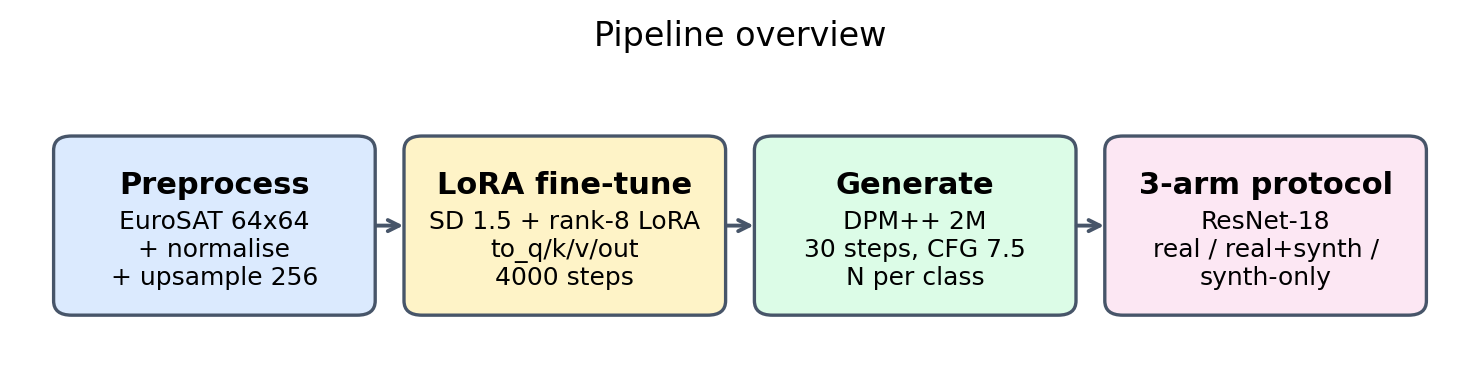
\includegraphics[width=0.95\linewidth]{figures/pipeline.png}\\[0.6em]
\footnotesize Four stages, end-to-end automated, evaluated by the canonical 3-arm protocol
of Frid-Adar et al.~\cite{fridadar2018gan}.
\end{frame}

% Slide 4 — Data + scope
\begin{frame}{Data and scope}
\textbf{Original plan:} xBD~\cite{gupta2019xbd} (flood/wildfire/pre-disaster) --- not approved within timebox.\\[0.4em]
\textbf{Actual:} EuroSAT~\cite{helber2019eurosat} 3-class proxy --- \texttt{forest}, \texttt{residential\_buildings}, \texttt{river}.

\vspace{0.6em}
\begin{tabular}{lccc}
\toprule
& train & val & test \\
\midrule
forest                & 2100 & 450 & 450 \\
residential\_buildings & 2100 & 450 & 450 \\
river                 & 1750 & 375 & 375 \\
\bottomrule
\end{tabular}
\vspace{0.4em}

Stratified 70/15/15 split, seed 42. Percentile normalisation (2/98); 64\,px native, upsampled to 256\,px for diffusion.
\end{frame}

% Slide 5 — Method: LoRA
\begin{frame}{Method: LoRA fine-tune of SD 1.5}
\textbf{What we train:} rank-8 LoRA on UNet cross-attention only --- \texttt{to\_q, to\_k, to\_v, to\_out.0}.
\vspace{0.4em}
\begin{itemize}
  \item $\sim$1.6\,M trainable parameters vs.\ 860\,M for the full UNet.
  \item Frozen: VAE, CLIP text encoder, the rest of the UNet.
  \item AdamW $\ell r = 10^{-4}$, cosine schedule, fp16 + grad checkpointing.
  \item Two budgets: \textbf{200 steps} (smoke), \textbf{4000 steps} (full --- adapter committed).
\end{itemize}
\vspace{0.6em}
\centering
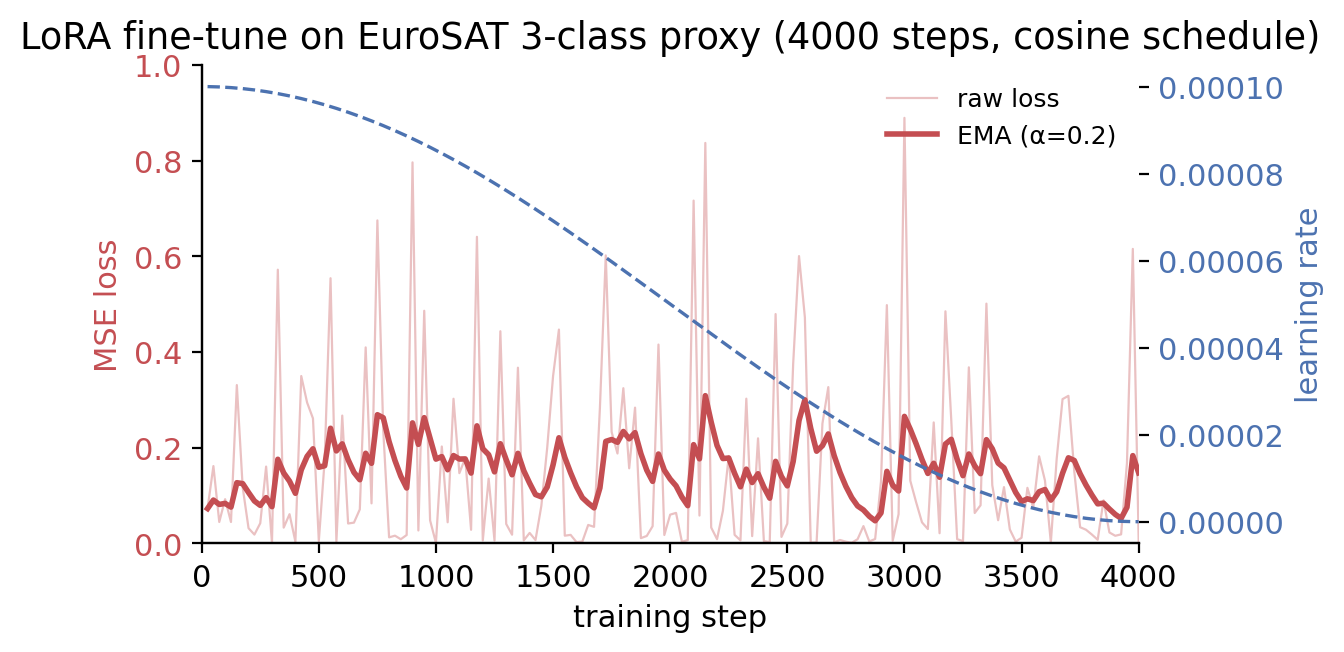
\includegraphics[width=0.78\linewidth]{figures/lora_loss_curve.png}
\end{frame}

% Slide 6 — Method: generation + 3-arm
\begin{frame}{Method: generation and three-arm protocol}
\textbf{Generation.} DPM++~2M Multistep, 30 inference steps, CFG 7.5, $256{\times}256$.
Deterministic per-image seeds, prompt template bank per class. Negative prompt
targets typical SD artefacts.

\vspace{0.4em}
\textbf{Three-arm classifier} (ResNet-18 ImageNet-pretrained, 64\,px):
\begin{enumerate}
\item \textbf{real-only}        --- baseline.
\item \textbf{real + synthetic} --- augmentation arm. Headline: $\Delta_\text{acc} = \text{arm2} - \text{arm1}$.
\item \textbf{synthetic-only}   --- sanity check.
\end{enumerate}
Same real-only test split across arms. Top-1 acc, macro-F1, weighted-F1.
\end{frame}

% Slide 7 — Quantitative results
\begin{frame}{Quantitative results --- 3-arm protocol}
\centering
\begin{tabular}{lccc}
\toprule
\textbf{Arm} & \textbf{acc} $\uparrow$ & \textbf{macro-F1} $\uparrow$ & \textbf{weighted-F1} $\uparrow$ \\
\midrule
1. real-only        & 0.9749 & 0.9744 & 0.9750 \\
2. real + synthetic & 0.9733 & 0.9726 & 0.9734 \\
3. synthetic-only   & 0.2706 & 0.2227 & 0.2176 \\
\midrule
\textbf{$\Delta$ (2 $-$ 1)} & \textbf{$-0.0016$} & \textbf{$-0.0017$} & \textbf{$-0.0016$} \\
\bottomrule
\end{tabular}
\vspace{0.6em}\\
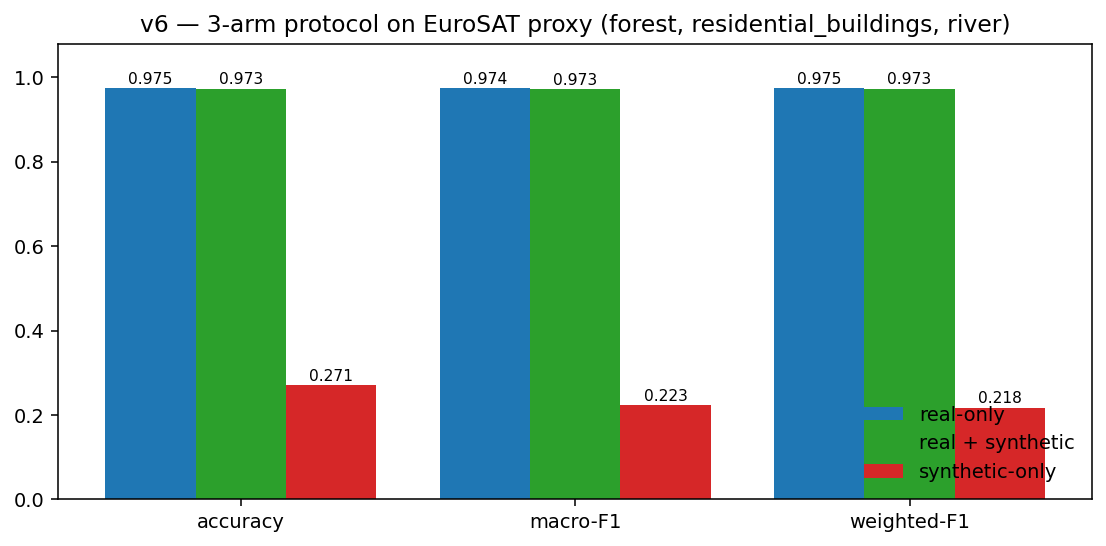
\includegraphics[width=0.72\linewidth]{figures/three_arm_overall.png}
\end{frame}

% Slide 8 — Qualitative
\begin{frame}{Qualitative: real vs.\ LoRA-generated}
\centering
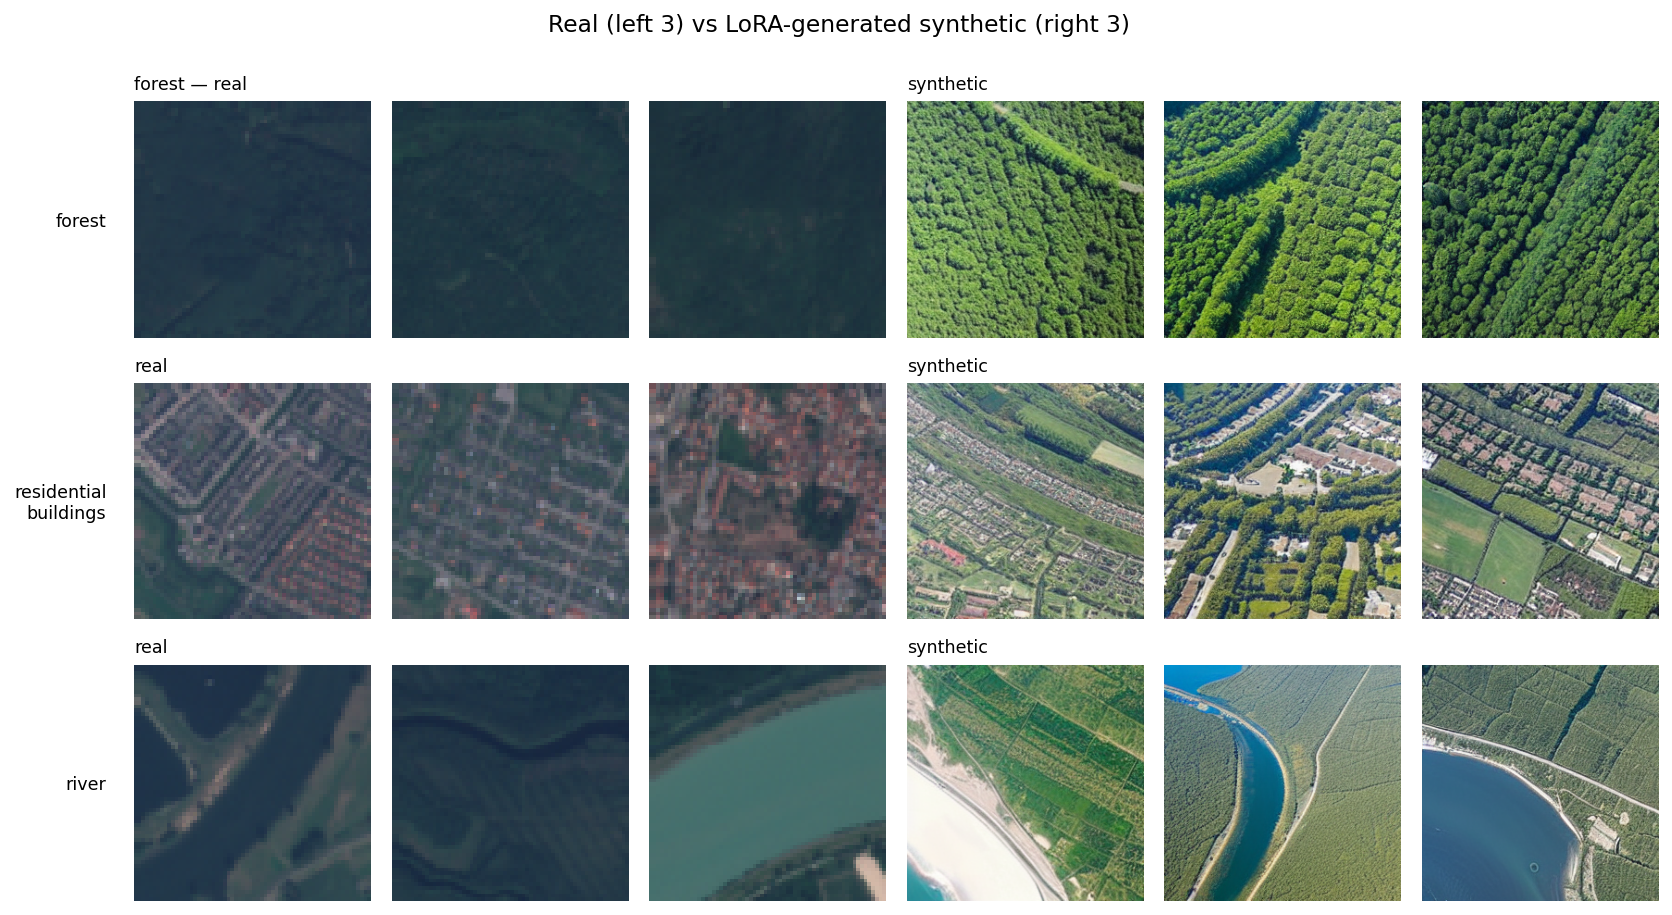
\includegraphics[width=0.92\linewidth]{figures/qualitative.png}\\[0.3em]
\footnotesize Left 3: real EuroSAT. Right 3: SD~1.5 + 200-step LoRA, 30 inference steps, $256{\times}256$.\\
Identifiable class structure; oversaturation and ``watercolour'' texture --- typical 200-step under-training.
\end{frame}

% Slide 9 — Interpretation, threats, future work
\begin{frame}{Interpretation, threats, future work}
\textbf{Interpretation.} $\Delta \approx 0$ on a saturated 0.975 baseline.
Consistent with Frid-Adar et al.~\cite{fridadar2018gan}: synthetic helps where real data is scarce / imbalanced; here it is not.
Synthetic-only at 0.27 (below 0.33 chance) quantifies the 200-step adapter's missing class-conditional signal.

\vspace{0.5em}
\textbf{Threats.} Proxy classes (not real disasters); single seed; under-trained adapter in the 3-arm; FID/SSIM not reported.

\vspace{0.5em}
\textbf{Future work.}
\begin{itemize}
\setlength\itemsep{-0.15em}
\item Inference for the 4000-step adapter on a non-Pascal GPU (we observed an SD 1.5 stall on Kaggle P100).
\item Multi-seed runs $\{42, 1337, 2024\}$ for mean $\pm$ std.
\item Apply to xBD's true disaster categories once access is granted.
\item Sweep synthetic-per-class $\in \{50, 100, 200, 400\}$.
\end{itemize}
\end{frame}

% Slide 10 — Conclusions + references
\begin{frame}[allowframebreaks]{Conclusions \& references}
\textbf{Contributions.}
\begin{itemize}
\setlength\itemsep{-0.15em}
\item Reproducible, fully open-source pipeline: preprocess $\to$ LoRA $\to$ generate $\to$ 3-arm.
\item 4000-step LoRA adapter on the EuroSAT 3-class proxy is shipped in the repository.
\item Empirical result on the saturated proxy: $\Delta_\text{acc} = -0.16\,\mathrm{pp}$ at the smoke configuration.
\item Honest scoping of the residual question (4000-step inference, disaster categories, seed variance).
\end{itemize}
\vspace{0.6em}
\centering
\footnotesize
\texttt{github.com/Aristogiannis/uniwa-computer-vision}\\
\texttt{notebooks/lora\_v7\_4000steps/} --- the 6.4\,MB adapter

\framebreak
\footnotesize
\begin{thebibliography}{9}
\bibitem{rombach2022highresolution} Rombach et al. \emph{High-Resolution Image Synthesis with Latent Diffusion Models}. CVPR 2022.
\bibitem{khanna2023diffusionsat} Khanna et al. \emph{DiffusionSat: A Generative Foundation Model for Satellite Imagery}. arXiv:2312.03606.
\bibitem{gupta2019xbd} Gupta et al. \emph{xBD: A Dataset for Assessing Building Damage from Satellite Imagery}. CVPR Workshops 2019.
\bibitem{fridadar2018gan} Frid-Adar et al. \emph{GAN-based synthetic medical image augmentation for increased CNN performance}. Neurocomputing 2018.
\bibitem{hu2021lora} Hu et al. \emph{LoRA: Low-Rank Adaptation of Large Language Models}. arXiv:2106.09685.
\bibitem{parmar2022cleanfid} Parmar et al. \emph{On Aliased Resizing and Surprising Subtleties in GAN Evaluation}. CVPR 2022.
\bibitem{helber2019eurosat} Helber et al. \emph{EuroSAT: A Novel Dataset and Deep Learning Benchmark for Land Use and Land Cover Classification}. JSTARS 2019.
\bibitem{ho2020ddpm} Ho et al. \emph{Denoising Diffusion Probabilistic Models}. NeurIPS 2020.
\bibitem{wang2004ssim} Wang et al. \emph{Image Quality Assessment: From Error Visibility to Structural Similarity}. IEEE TIP 2004.
\end{thebibliography}
\end{frame}

\end{document}
